\documentclass{article}

\usepackage[margin=0.75in]{geometry}
\usepackage{graphicx}
\usepackage{multicol}
\usepackage{lipsum}
\usepackage[colorlinks]{hyperref}
\usepackage{pgfplots}
\pgfplotsset{compat=1.16}

\begin{document}

\begin{multicols}{2}
  \begin{flushleft}
    \Huge
    Your personal results\\for the Christian Life Survey
  \end{flushleft}
  \columnbreak
  
\includegraphics{c4se-logo}
\end{multicols}

\section*{Introduction}
\lipsum[1-2]

\section*{Spiritual Foci}
\lipsum[3-4]

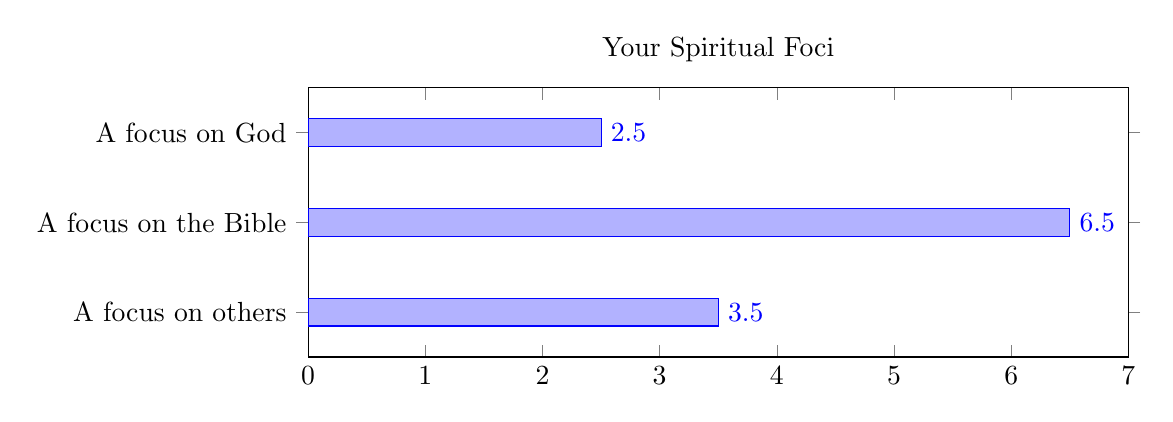
\begin{tikzpicture}
  \begin{axis}[
    title=Your Spiritual Foci,
    xbar, xmin=0, xmax=7,
    width=12cm,
    height=5cm,
    enlarge y limits=0.25,
    symbolic y coords={A focus on others,A focus on the Bible,A focus on God},
    ytick=data,
    nodes near coords,
    nodes near coords align={horizontal},
    ]
    \addplot coordinates {
      (3.5,A focus on others)
      (2.5,A focus on God)
      (6.5,A focus on the Bible)
    };
  \end{axis}
\end{tikzpicture}

\section*{Spiritual Orientations}
\lipsum[4-6]

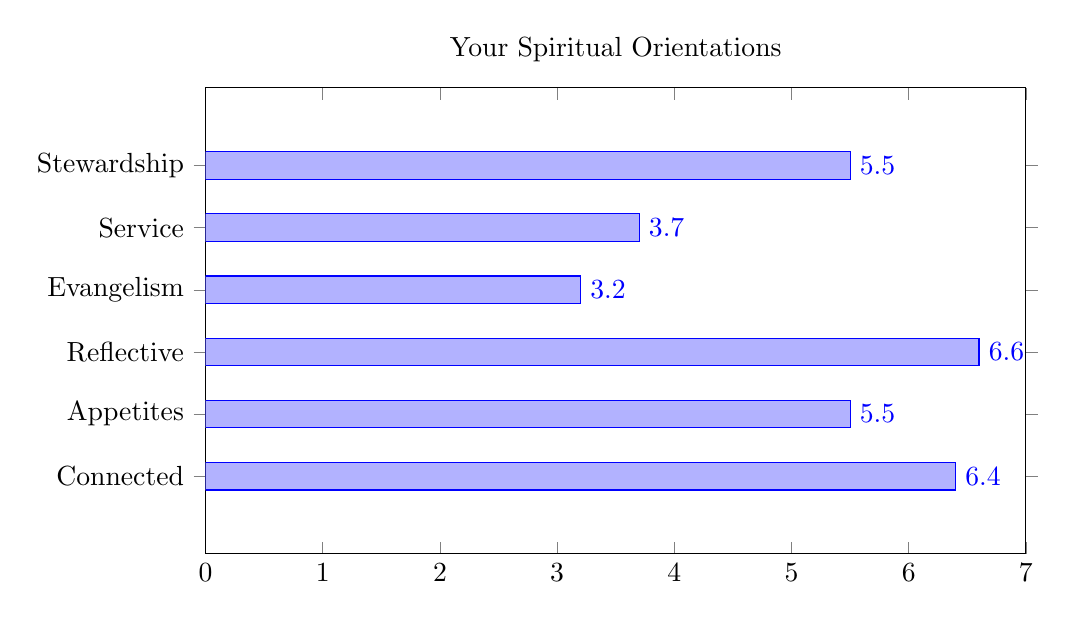
\begin{tikzpicture}
  \begin{axis}[
    title=Your Spiritual Orientations,
    xbar, xmin=0, xmax=7,
    width=12cm,
    height=7.5cm,
    enlarge y limits=0.25,
    symbolic y coords={Connected,Appetites,Reflective,Evangelism,Service,Stewardship},
    ytick=data,
    nodes near coords,
    nodes near coords align={horizontal},
    ]
    \addplot coordinates {
      (6.4,Connected)
      (5.5,Appetites)
      (6.6,Reflective)
      (3.2,Evangelism)
      (3.7,Service)
      (5.5,Stewardship)
    };
  \end{axis}
\end{tikzpicture}


\section*{Scripture Engagement}
\lipsum[5]
\subsection*{Explanation}
\lipsum[6-7]
\subsection*{Results}
\lipsum[8]

\section*{More Information}
\lipsum[2]
\begin{center}
  \vspace{0.25in}
  \href{http://tucse.taylor.edu/}{
\includegraphics{c4se-logo}}

  \vspace{0.25in}
  \href{http://tucse.taylor.edu/}{Taylor University Center for Scripture Engagement}

  \vspace{0.25in}
  \href{https://www.biblegateway.com/resources/scripture-engagement/}{Bible Engagement at Bible Gateway }
\end{center}

\end{document}

%%% Local Variables:
%%% mode: latex
%%% TeX-master: t
%%% End:
